\chapter{Metodología}

En este capítulo ahondaremos en los conceptos más importantes que hemos de entender de cara al funcionamiento de nuestro modelo generativo, tanto en el entrenamiento como en la generación de comentarios.



\section{Datos de entrada y preprocesamiento}
En primer lugar, debemos ofrecer los datos de entrada al modelo. Estos datos deben estar previamente formateados y unificados. Veamos cómo se ha acometido dicho preprocesamiento.

En la Sección \ref{sec:preprocess} expondremos los diferentes métodos y técnicas utilizadas de preprocesamiento de texto para darle una forma apropiada y unificada al conjunto de datos, antes de poder introducirlos en el modelo.

En la Figura \ref{fig:preprocess-diagram} se ilustra un esquema de los pasos a seguir en dicha fase del proyecto. Explicaremos cada paso desde el punto de vista de los dos conjuntos de datos a unificar, ya que cada uno necesitará de un tratamiento particular en función de su etado inicial.

\begin{figure}[h!]
	\centering
	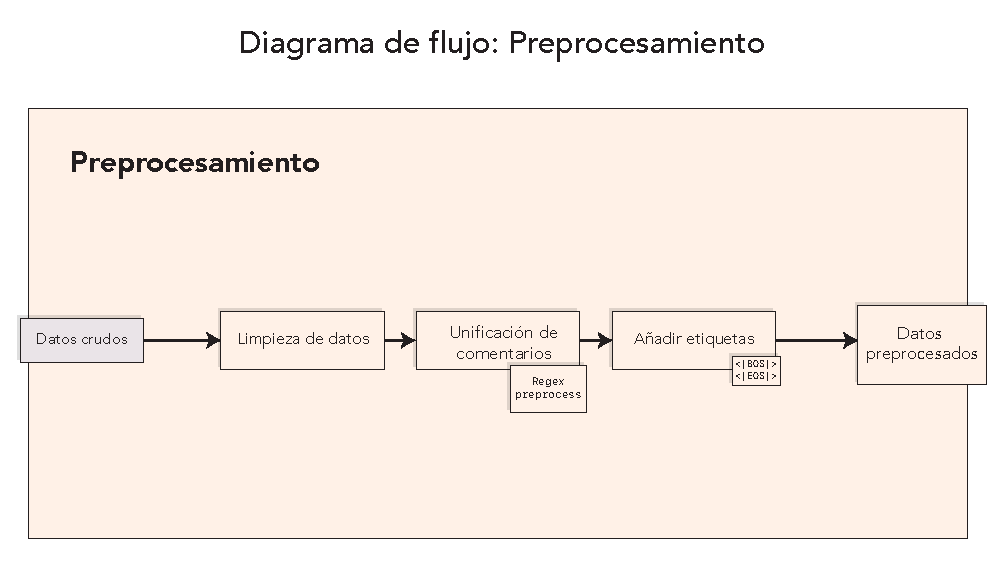
\includegraphics[width=.9\textwidth]{media/preprocess.pdf}
	\caption{Diagrama resumen del preprocesamiento efectuado en los datos.}
	\label{fig:preprocess-diagram}
\end{figure}


Es importante la adición de las etiquetas \jesitt{<|BOS|>} y \jesitt{<|EOS|>}. Estas etiquetas son las siglas de \textit{begin of sentence} y \textit{end of sentence}. Son marcadores que indican el inicio y fin de una oración. Estas etiquetas son necesarias para que el modelo entienda cuál es el criterio a partir del cual empieza y acaba una oración.

\subsection{Codificación de los tokens}
Antes de pasar los datos al modelo, debemos codificarlos. Codificar significa obtener un código único en función del token que estemos considerando. La codificación es esencial para estos modelos, ya que ofrece una representación matemática de las palabras. La codificación de los tokens se efectúa mediante un diccionario preentrenado, de forma que la codificación y decodificación sean consistentes, dado un modelo determinado.

Este proceso es relativamente simple: para cada palabra que encontremos en el texto, le asociamos un índice y guardamos la entrada en un diccionario. De esta forma, cada vez que queramos que la red procese un extracto de texto, sustituimos cada término por su correspondiente número en el diccionario. De esta tarea también se suele encargar el Tokenizer. 

Como vimos en la Sección \ref{sec:tokens}, estos algoritmos solo se encargan de transformar el texto en vectores, pero al ser una tarea perteneciente a la fase de preprocesamiento, las librerías suelen ofrecer esta funcionalidad de forma conjunta. Esto también garantiza que el tokenizer utilizado para un determinado modelo sea el mismo de una ejecución a otra, ya que de otra forma habría problemas con la codificación.

\begin{figure}[h]
	\centering
	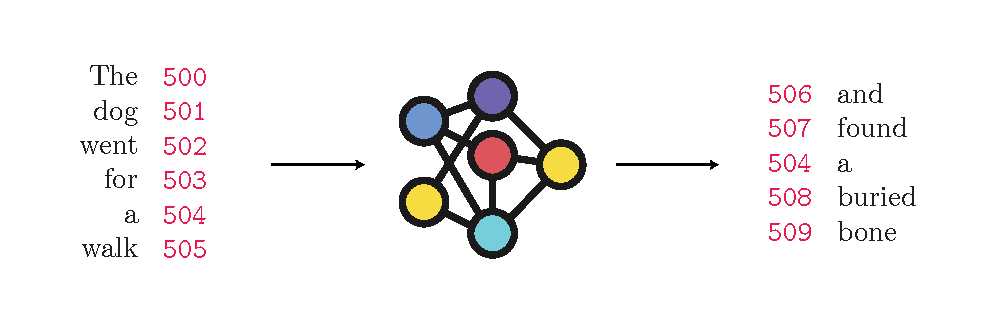
\includegraphics[width=.9\textwidth]{media/tokenizer.pdf}
	\caption{Ilustración del proceso de codificación -- decodificación necesario}
	\label{fig:codification}
\end{figure}

Una vez procesado, el modelo nos devolverá una secuencia de números, de los que podemos volver a obtener el texto subyacente deshaciendo la operación.




\section{Ajuste de los pesos}
\begin{figure}[h]
	\centering
	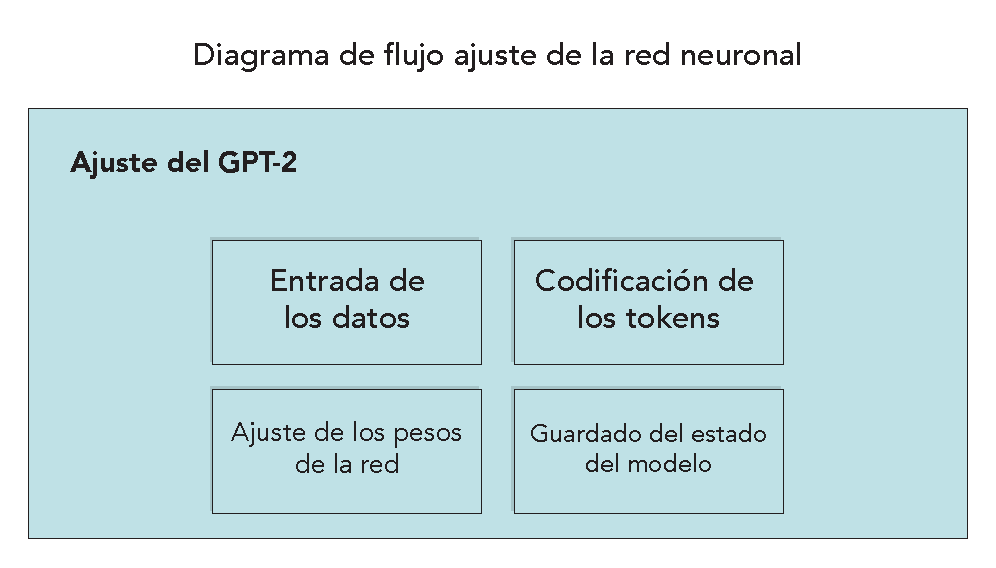
\includegraphics[width=.9\textwidth]{media/gpt-fine-tune.pdf}
	\caption{Diagrama resumen del ajuste de los pesos del GPT-2}
	\label{fig:fine-tune-gpt}
\end{figure}

Nuestro modelo ya está construido. Esto es, los diseñadores ya han decidido las distintas capas y el orden de estas según hemos visto en las secciones anteriores. Este modelo se nos ofrece preentrenado de forma bastante simple. Tal y como viene en el paquete, es capaz de generar frases con relativo sentido, es decir, de algún modo \textit{sabe hablar}. 

El ajuste se efectúa como un proceso de aprendizaje no supervisado, en la que exponemos a la red a un conjunto de comentarios de forma que ésta podrá generar nuevos comentarios que caigan bajo la función de distribución de los comentarios de entrada. 

En nuestro caso, esta función de distribución la define nuestro conjunto de datos de informes médicos. Este proceso efectivamente ajusta los pesos de la red de forma que se familiarice al modelo con el vocabulario y expresiones comunes encontradas en los extractos médicos presentados.

Este proceso es, computacionalmente, extraordinariamente costoso. Debemos calcular el peso de millones de parámetros (117 millones en nuestro caso particular), debido a la magnitud del modelo. Para ello, hemos de tener disponible un equipo con, como mínimo, una tarjeta gráfica decente que nos permita hacer cálculos matriciales en paralelo, operaciones muy comunes en el entrenamiento de las redes neuronales.

Dichos equipos pueden ser muy caros. Para ello, hicimos uso del servicio de clústeres del Instituto DaSCI. En dicho servicio se nos puede asignar una máquina dependiendo de la carga que tengan las demás. Por referencia, \textbf{Selene}, uno de los equipos disponibles, consta de:
\begin{itemize}
	\item \textbf{Procesador}: Dual 20-Core Intel Xeon E5-2698 v4 2.2 GHz
	\item \textbf{RAM}: 512 GB 2,133 MHz DDR4 RAM
	\item \textbf{Disco}: 4 $\times$ 1.92 TB SSD RAID 0
	\item \textbf{Gráfica}: 8 $\times$ GPU NVIDIA Tesla V100 32GB 
\end{itemize}

Mediante \jesitt{ssh}, nos conectamos a la máquina que el equipo nos haya asignado y enviamos nuestros archivos usando \jesitt{scp}. Una vez nuestros archivos están en la máquina de destino, entrenamos el modelo, obtenemos los pesos y los descargamos de vuelta de la misma forma.

Gracias a las bibliotecas \jesitt{pytorch}\cite{pytorch} y \jesitt{transformers}\cite{WolfEtal2020Transformers}, podemos reentrenar nuestro modelo GPT-2 con nuestros datos, como se puede ver en \href{https://huggingface.co/transformers/custom_datasets.html}{Fine-tuning with custom datasets}. 

\subsection{Guardado del estado del modelo}
Finalmente, una vez entrenado el modelo, lo más importante es guardar su estado. Mediante la función \jesitt{torch.save()}, podemos determinar el lugar en el que el estado del modelo se guardará. Este estado se guarda en un archivo, que, generalmente, consta de un diccionario en el que las claves corresponden a los nodos de las capas en sí, es decir, a sus parámetros entrenables, y cuyo valor es el peso de dicho nodo. 

De la misma forma, mediante \jesitt{torch.load()}, podemos cargar un modelo \textit{vacío} con los pesos del archivo que especifiquemos, sobreescribiendo los valores por defecto y efectivamente recuperando el estado en el que dejamos el modelo tras el entrenamiento.



\section{Generación de comentarios}

\begin{figure}[h]
	\centering
	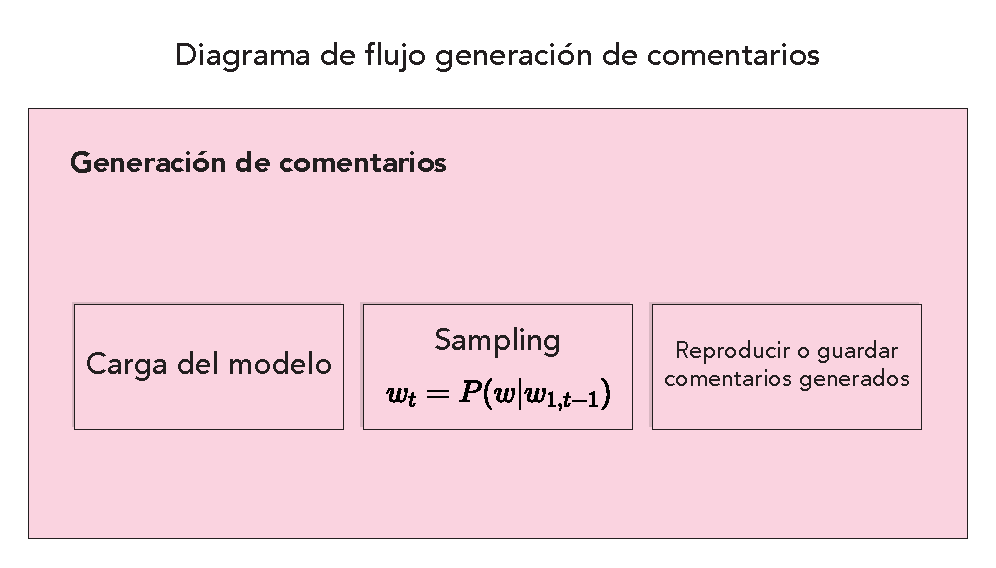
\includegraphics[width=.9\textwidth]{media/comment-gen.pdf}
	\caption{Diagrama resumen de la generación de comentarios}
	\label{fig:comment-gen}
\end{figure}

En esta sección hablaremos de la generación de comentarios, una vez nuestro modelo está entrenado y listo para funcionar. 

\subsection{Carga del modelo}
Con nuestro archivo con los pesos localizado, podemos cargar de vuelta los pesos relevantes en los parámetros correspondientes de la red, recuperando el estado original. Este estado es el que nos permitirá generar comentarios de forma automática.

\subsection{Sampling y otros métodos de generación de texto}
Una vez entrenado el modelo y ajustados los pesos, ya tenemos un marco de trabajo sobre el que poder generar comentarios de texto libre. Aun así, el modelo no es capaz de ofrecernos inferencias como en modelos clásicos de predicción o clasificación. Para poder acometer el proceso de generación de palabras, debemos efectuar una \textit{decodificación} de las mismas, y existen varias formas para acometer esto. 


Existen varias maneras de generar lo que en la jerga se denomina \textit{texto abierto}, es decir, generar texto de forma relativamente libre y sin restricciones. Muchos otros modelos son capaces de hacerlo, aunque nosotros nos centraremos en los métodos que conciernen a nuestro GPT-2, que es un modelo autorregresivo.

Los modelos autorregresivos asumen que la siguiente palabra a generar se calcula como una función de probabilidad de todas las palabras anteriores, dada una palabra de contexto inicial. Dicho esto, existen varias maneras de \textit{decodificar} texto de un modelo de lenguaje. Veamos las más relevantes.

Los métodos de decodificación aquí mencionados aparecen en la publicación \href{https://huggingface.co/blog/how-to-generate}{How to generate text} de Patrick von Platen. Es uno de los integrantes de Hugging Face, una de las empresa de código abierto que se dedica a la creación de los diferentes modelos mencionados anteriormente, desarrolladores de la librería \jesitt{transformers}, entre otras.

\subsubsection{Greedy search y beam search}
La búsqueda voraz obtiene la palabra con mayor probabilidad de todas las opciones dada una palabra inicial. 


\begin{figure}[h]
	\centering

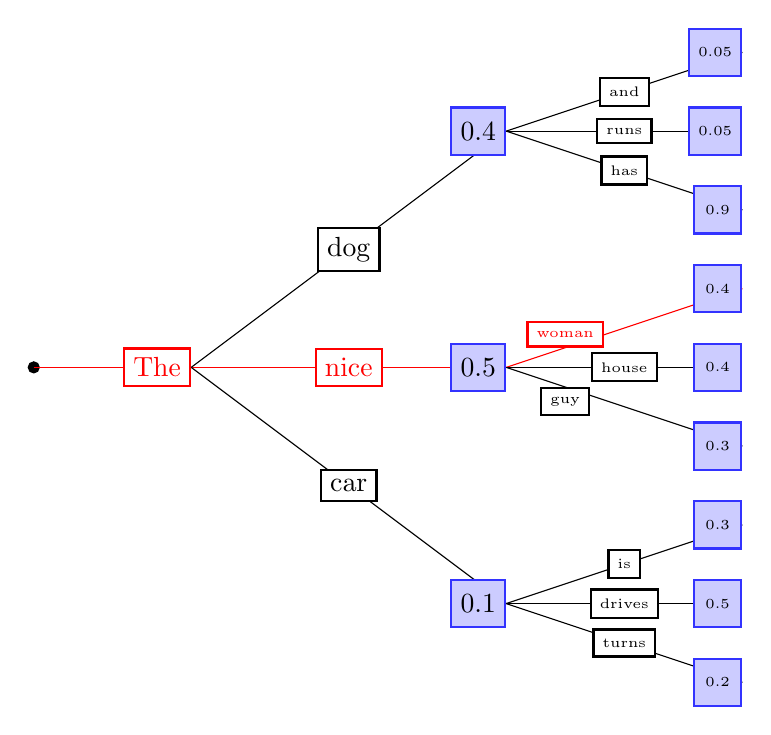
\begin{tikzpicture}
	\tikzstyle{tag}=[shape=rectangle,thick,draw,fill=white,minimum size=0.3cm]
	\tikzstyle{ntag}=[shape=rectangle,thick,draw=blue!80,fill=blue!20,minimum size=0.6cm]

	\filldraw [black] (-4,0) circle (2pt);
	
	
	%%%
	\draw (-2,0) -- node[tag] {dog} (2,3);
	\draw[red] (-2,0) -- node[tag] {nice} (2,0);
	\draw (-2,0) -- node[tag] {car} (2,-3);
	
	\node at (2, 3) [ntag, anchor= east] {0.4};
	\node at (2, 0) [ntag, anchor= east]{0.5};
	\node at (2, -3) [ntag, anchor= east]{0.1};
	
	
	%%%
	\draw[red] (2,0) -- node[tag, near start, anchor=south] {\tiny woman} (5,1);
	\draw (2,0) -- node[tag] {\tiny house} (5,0);
	\draw (2,0) -- node[tag, near start, anchor=north] {\tiny guy} (5,-1);
	
	
	
	\node at (5, 1) [ntag, anchor= east] {\tiny 0.4};
	\node at (5, 0) [ntag, anchor= east]{\tiny 0.4};
	\node at (5, -1) [ntag, anchor= east]{\tiny 0.3};
	
	%%%
	\draw (2,3) -- node[tag] {\tiny and} (5,4);
	\draw (2,3) -- node[tag] {\tiny runs} (5,3);
	\draw (2,3) -- node[tag] {\tiny has} (5,2);
	
	\node at (5, 4) [ntag, anchor= east] {\tiny 0.05};
	\node at (5, 3) [ntag, anchor= east]{\tiny 0.05};
	\node at (5, 2) [ntag, anchor= east]{\tiny 0.9};
	
	%%%
	\draw (2,-3) -- node[tag] {\tiny is} (5,-2);
	\draw (2,-3) -- node[tag] {\tiny drives} (5,-3);
	\draw (2,-3) -- node[tag] {\tiny turns} (5,-4);
	
	\node at (5, -2) [ntag, anchor= east] {\tiny 0.3};
	\node at (5, -3) [ntag, anchor= east]{\tiny 0.5};
	\node at (5, -4) [ntag, anchor= east]{\tiny 0.2};


	\draw[red] (-4,0) -- (-2,0)
	node[tag, anchor=east] {The};
\end{tikzpicture}

	\caption{Ilustración de los pasos que daría el algoritmo greedy, tomando siempre la posibilidad más alta. Se muestra en rojo el camino que el algoritmo tomaría en este particular ejemplo, ya que \textit{nice} supera a los otros dos términos en la probabilidad de ser elegido.}
	\label{tkz:greedy}
\end{figure}

Dada una palabra inicial que tomamos del usuario, por ejemplo, siempre tomaremos aquella palabra de todas las posibles opciones que más probabilidad tenga de aparecer, dada la palabra anterior. Dichas probabilidades se calculan en el entrenamiento del modelo. Podemos ver un ejemplo de este comportamiento en la Figura \ref{tkz:greedy}.

El algoritmo toma siempre la palabra más probable y esto funcionará bien, aunque este algoritmo peca de empezar a repetirse bastante pronto. Esto es, generará secuencias que contienen palabras finales e iniciales similares, por lo que el ciclo empieza de nuevo al escogerse siempre la palabra más probable.



\begin{figure}[h!]
	\centering
	
	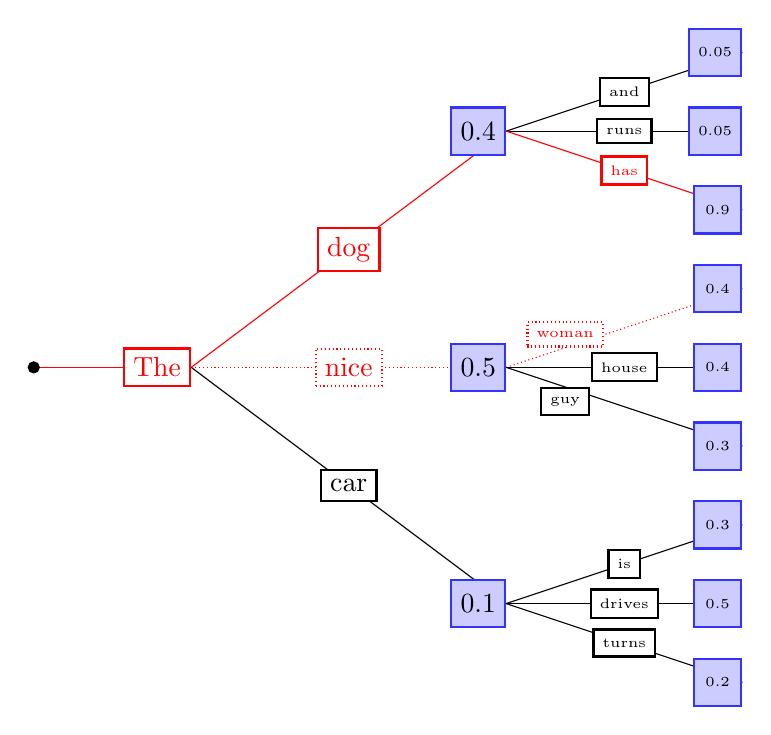
\begin{tikzpicture}
		\tikzstyle{tag}=[shape=rectangle,thick,draw,fill=white,minimum size=0.3cm]
		\tikzstyle{ntag}=[shape=rectangle,thick,draw=blue!80,fill=blue!20,minimum size=0.6cm]
		
		
		\draw[red] (-4,0) -- (-2,0)
		node[tag, anchor=east] {The};
		
		\filldraw [black] (-4,0) circle (2pt);
		
		
		%%%
		\draw[red] (-2,0) -- node[tag] {dog} (2,3);
		\draw[red, densely dotted] (-2,0) -- node[tag] {nice} (2,0);
		\draw (-2,0) -- node[tag] {car} (2,-3);
		
		\node at (2, 3) [ntag, anchor= east] {0.4};
		\node at (2, 0) [ntag, anchor= east]{0.5};
		\node at (2, -3) [ntag, anchor= east]{0.1};
		
		
		%%%
		\draw[red, densely dotted] (2,0) -- node[tag, near start, anchor=south] {\tiny woman} (5,1);
		\draw (2,0) -- node[tag] {\tiny house} (5,0);
		\draw (2,0) -- node[tag, near start, anchor=north] {\tiny guy} (5,-1);
		
		
		
		\node at (5, 1) [ntag, anchor= east] {\tiny 0.4};
		\node at (5, 0) [ntag, anchor= east]{\tiny 0.4};
		\node at (5, -1) [ntag, anchor= east]{\tiny 0.3};
		
		%%%
		\draw (2,3) -- node[tag] {\tiny and} (5,4);
		\draw (2,3) -- node[tag] {\tiny runs} (5,3);
		\draw[red] (2,3) -- node[tag] {\tiny has} (5,2);
		
		\node at (5, 4) [ntag, anchor= east] {\tiny 0.05};
		\node at (5, 3) [ntag, anchor= east]{\tiny 0.05};
		\node at (5, 2) [ntag, anchor= east]{\tiny 0.9};
		
		%%%
		\draw (2,-3) -- node[tag] {\tiny is} (5,-2);
		\draw (2,-3) -- node[tag] {\tiny drives} (5,-3);
		\draw (2,-3) -- node[tag] {\tiny turns} (5,-4);
		
		\node at (5, -2) [ntag, anchor= east] {\tiny 0.3};
		\node at (5, -3) [ntag, anchor= east]{\tiny 0.5};
		\node at (5, -4) [ntag, anchor= east]{\tiny 0.2};
		
	
\end{tikzpicture}

	\caption{Ilustración demostrando el funcionamiento del \textit{beam search}, con 2 beams en este caso. Vemos como se toman dos caminos, en línea continua el camino definitivo y en línea discontinua la otra alternativa. La probabilidad conjunta del camino elegido es $0.4 \times 0.9 = 0.36$, en contraste con el camino alternativo cuya probabilidad es de $0.5 \times 0.4 = 0.2$. Se toma un camino que a priori no es tan probable pero que a largo plazo, sí.}
	\label{tkz:beams}
\end{figure}


Una solución planteada es el \textit{beam search}, que podemos visualizar en la Figura \ref{tkz:beams}, algo así como una búsqueda distribuida. Dadas las probabilidades de cada palabra, el algoritmo calcula varios pasos en avanzadilla para varias alternativas, y devuelve aquella secuencia que más probabilidad general tenga. Esto soluciona algunos problemas, pero no termina de lidiar con el factor de repetitividad anterior. 

Por otro lado, Ari Holtzmann sugiere en \cite{holtzman2020curious} que la generación del lenguaje humano no se guía por la elección de las palabras más probables. El lenguaje humano real es mucho menos predecible, ya que de otra forma sería \textit{aburrido} de leer o escuchar.

Es por ello que los métodos alternativos han de evitar las técnicas \textbf{deterministas} de generación de texto, y apostar por los métodos con gran influencia aleatoria.

\subsubsection{Sampling}

Sampling es otra técnica de generación de lenguaje autorregresiva. En la forma más básica, el muestreo simplemente toma una palabra de forma aleatoria, ponderándolas con una distribución de probabilidad tal que:

\begin{equation}
	w_t = P(w | w_{1, t-1})
\end{equation}

es decir, la probabilidad de escoger la palabra $w_t$ depende de todas las palabras anteriores.

\begin{figure}[h]
	\centering
	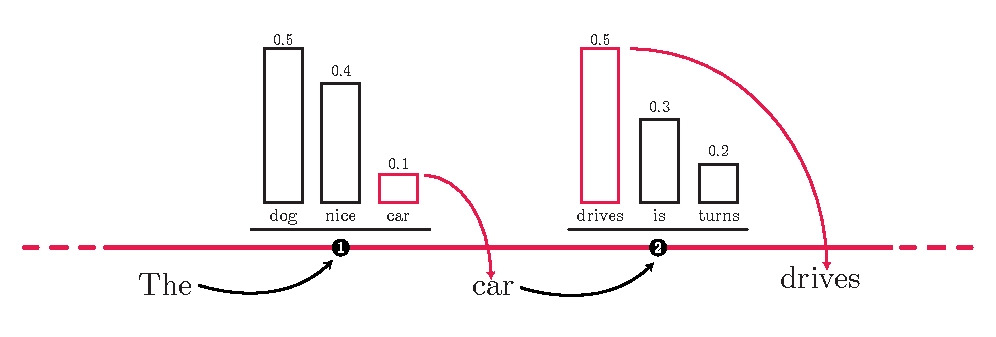
\includegraphics[width=.9\textwidth]{media/sampling.pdf}
	\caption{Ilustración de un ejemplo de muestreo. Se toman palabras aleatoriamente, aunque se pondera en función de su probabilidad.}
	\label{fig:sampling}
\end{figure}

El hecho de que una palabra presente una gran probabilidad de ser escogida no corresponde con que al final se la acabe escogiendo, como vemos en el paso 1 de la Figura \ref{fig:sampling}. En este caso, se escogió \textit{car} y posteriormente sí se escogió la palabra más probable. Este proceso nos ayuda a explorar más el espacio de búsqueda subyacente compuesto de todas las combinaciones de palabras posibles.

\subsubsection{Temperatura}
Podemos graduar la ponderación de la que hablamos con lo que los autores denominan la \textit{temperatura} de la función de activación \textit{softmax} de la última capa del modelo.

Al bajar la temperatura por debajo de 1 (siendo 1 un ajuste nulo), las palabras más probables se saturan, es decir, se hacen más probables, y las menos probables se comprimen, haciéndolas menos probables. En el otro extremo, al ajustar la temperatura a límites muy cercanos a 0, nos encontraríamos con la búsqueda voraz de la que hablamos antes.

Este factor nos ofrece una especie de regulador entre \textbf{máximo determinista} o \textbf{máximo aleatorio}.

La adición de esta técnica ayuda a que la generación no sea \textit{extremadamente} aleatoria. Si bien en la sección anterior comentábamos que debíamos añadir aleatoriedad, todo en exceso es malo. Una generación completamente aleatoria es, en su mayoría, poco coherente. La bajada sutil de la temperatura del modelo provoca que se elijan, normalmente, palabras bastante probables, pero que de vez en cuando se escojan palabras poco probables. Dichas palabras ahora abren nuevos caminos por los que continuar generando, que no hubieran sido considerados de otra forma, pero continuamos eligiendo, por lo general, combinaciones de palabras más probables, para garantizar la coherencia del texto.

En esencia, el proceso es un gran compromiso entre coherencia y predecibilidad, además de los demás grandes problemas presentes como los bucles infinitos.

\subsubsection{Top K Sampling}

Dadas las premisas anteriores, las siguientes técnicas son mejoras incrementales que tratan de solucionar algunos otros problemas existentes.

El muestreo de los K mejores, tal y como su nombre indica, solo considera las K mejores opciones de toda la batería de palabras posibles. Dado este subconjunto K, se muestrea una palabra como en el Sampling original, tomándola aleatoriamente de forma ponderada. Puede verse en la Figura \ref{fig:top-k} 


\begin{figure}[h]
	\centering
	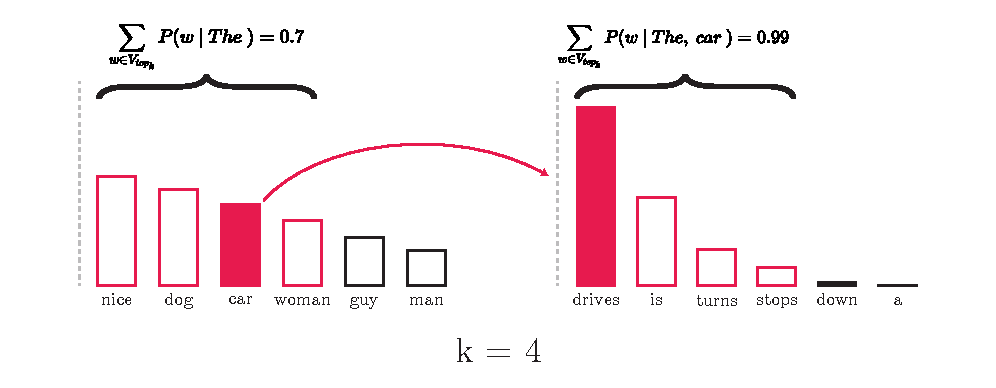
\includegraphics[width=.9\textwidth]{media/top k.pdf}
	\caption{Ilustración del proceso de cálculo en muestreo con un valor de $k = 4$.}
	\label{fig:top-k}
\end{figure}

Esta técnica elimina posibles elecciones bastante malas, lo que Holtzmann denomina como "\textit{the unreliable tail}", que podemos acuñar como \textit{la cola traicionera}, que puede observarse en la ilustración. Holtzmann afirma que existe una enorme cantidad de palabras con muy baja probabilidad en cada elección que, en realidad, están sobrerepresentadas cuando hablamos de términos agregados. Es decir, la \textbf{probabilidad agregada} de todas esas palabras con una bajísima probabilidad puede corresponder a \textbf{grandes proporciones de la distribución de probabilidad}, lo que, efectivamente, va en contra de nuestro objetivo.

Tomando solo aquellas K mejores, se elimina dicha cola y se redistribuye la probabilidad de los términos elegidos de forma oportuna, creando un modelo de decodificación mucho más natural que los otros.

\subsubsection{Top P nucleus}

Finalmente, esta última técnica se denomina Top P nucleus, refiriéndose a un valor diferente al K anterior.

En este caso, en lugar de tomar los K mejores términos, tomamos el conjunto más pequeño de términos cuya probabilidad acumulada supere el $p$ establecido por el usuario. Esto es, dado un $p = 0.9$, tomamos las $n$ mejores palabras que, dada la suma de su probabilidad, se supere el $p$ determinado. El proceso es básicamente idéntico al ilustrado en la Figura \ref{fig:top-k}, solo que consideramos la probabilidad acumulada, no un número de términos.

Esto provoca que en lugar de tomar un subconjunto de palabras de cardinalidad constante durante todo el proceso, ahora el tamaño varía. Se ha demostrado que esta flexibilidad ayuda y contribuye a una generación de texto más natural.

\vspace{15mm}
Estos dos últimos métodos son los más utilizados en el estado del arte, y este último es el que \textbf{utilizamos nosotros} en nuestro proyecto a la hora de generar palabras. Como vemos, aun disponiendo de una red neuronal muy potente, no es trivial extraer información coherente y de calidad.